% chapterquote command.
\newcommand{\chapterquote}[2] {
\begin{quote}
\textit{"{#1}"}

--- {#2}
\end{quote}
\vspace{12pt}
}


\documentclass[a4paper,10pt]{report}
\usepackage{graphicx}
\usepackage{listings}
\usepackage{chngpage}


\begin{document}

\newpage
\changepage{60mm}{}{}{-39mm}{}{-45mm}{}{}{}

\renewcommand\thepage{}

\begin{center}
    
\includegraphics{gfx/chalmers-header.eps}
\end{center}

\vspace{60mm}

\begin{adjustwidth}[]{20mm}{-40mm}
    {\LARGE \textbf{Investigating storage solutions for large data}}

    \vspace{6pt}

    \noindent {\Large \textit{A comparison of well performing and scalable data storage \\ 
                              solutions for real time extraction and batch insertion of data }}
    \vspace{6pt}

    \noindent {\large \textit{Master of Science Thesis}}

    \vspace{36pt}
    
    \noindent {\Large \textbf{ADAM LITH}}

    \noindent {\Large \textbf{JAKOB MATTSSON}}
    
    \vfill

    \noindent Department of Computer Science and Engineering

    \noindent CHALMERS UNIVERSITY OF TECHNOLOGY

    \noindent G{\"o}teborg, Sweden, 2010
\end{adjustwidth}

\newpage
\renewcommand\thepage{\arabic{page}}
\changepage{-60mm}{}{}{39mm}{}{47mm}{}{}{}

\pagebreak

\setcounter{page}{1}

\noindent The Author grants to Chalmers University of Technology and University of Gothenburg the non-exclusive right to publish the Work electronically and in a non-commercial purpose make it accessible on the Internet.

\vspace{12pt}

\noindent The Author warrants that he/she is the author to the Work, and warrants that the Work does not contain text, pictures or other material that violates copyright law.

\vspace{12pt}

\noindent The Author shall, when transferring the rights of the Work to a third party (for example a publisher or a company), acknowledge the third party about this agreement. If the Author has signed a copyright agreement with a third party regarding the Work, the Author warrants hereby that he/she has obtained any necessary permission from this third party to let Chalmers University of Technology and University of Gothenburg store the Work electronically and make it accessible on the Internet.

\vspace{64pt}

\noindent Investigating storage solutions for large data

\vspace{24pt}

\noindent ADAM LITH

\noindent JAKOB MATTSSON

\vspace{12pt}

\noindent {\copyright} ADAM LITH, June 2010

\noindent {\copyright} JAKOB MATTSSON, June 2010

\vspace{12pt}

\noindent Examiner: GRAHAM KEMP

\vspace{72pt}

\noindent Department of Computer Science and Engineering

\noindent Chalmers University of Technology

\noindent SE-412 96 G{\"o}teborg

\noindent Sweden

\noindent Telephone + 46 (0)31-772 1000

\vfill

\noindent Department of Computer Science and Engineering

\noindent G{\"o}teborg, Sweden, 2010

\pagebreak

\noindent {\Large \textbf{Abstract}}
\vspace{12pt}

\noindent There are several systems developed today to handle the problem of storing large amounts of data. But for each type of data and set of operations different systems differ in suitability. Burt AB stores a large dataset, enlarged in batches in a regular and controlled way, but never updated. Query times are critical and must have real-time performance.

This thesis describes a systematic exploration and testing of possible solutions, with the goal of recommending one of these for Burt AB. Inherent properties of the dataset itself are investigated and a set of very different database management systems are combined with a set of database schemas in order to form a total of eleven potential solutions of interest.

We show that the relational model suits the data well and that the maturity of MySQL gives us confidence when recommending it compared to the more recently developed systems. Furthermore, indexing using an inverted index is found to yield the best results.

\vspace{48pt}

\noindent {\Large \textbf{Sammanfattning}}
\vspace{12pt}


\noindent Det finns ett stort antal system som utvecklats f{\"o}r att l{\"o}sa problemet med att hantera mycket data, men vilken l{\"o}sning som {\"a}r b{\"a}st beror p{\aa} vilken typ av data man har. Burt AB hanterar en stor datam{\"a}ngd som fylls p{\aa} med mycket ny data p{\aa} ett regelbundet och kontrollerat s{\"a}tt, men aldrig uppdateras. L{\"a}sning av datan m{\aa}ste dock kunna ske i realtid.

Denna uppsats beskriver en systematisk utforskning och testning av m{\"o}jliga l{\"o}sningar, med m{\aa}let att rekomendera en av dessa f{\"o}r Burt AB. Egenskaper hos datan sj{\"a}lv unders{\"o}ks, och en handfull v{\"a}ldigt olika databashanteringssystem {\"a}r kombinerade med olika datasscheman f{\"o}r att skapa totalt elva olika potentiella l{\"o}sningar.

Vi visar att relationsmodeller passar datan v{\"a}l, och att mognadsniv{\aa}n hos MySQL ger den ett {\"o}vertag gentemot andra mer nyligen utvecklade system. Ut{\"o}ver detta s{\aa} visar det sig att inverterade index {\"a}r den b{\"a}st l{\"a}mpade l{\"o}sningen f{\"o}r bra resultat.

\pagebreak

\noindent {\Large \textbf{Preface}}
\vspace{12pt}

\noindent Adam Lith and Jakob Mattsson both study Computer Science at Chalmers University of Technology in Gothenburg, Sweden. This thesis is part of their master's degree. The work was performed at Burt's office in Gothenburg during spring 2010.

\vspace{24pt}

\noindent \textbf{Acknowledgements}
\vspace{12pt}

\noindent The authors would like to especially thank the supervisors---Graham Kemp at Chalmers and John Sj{\"o}lander at Burt---for their help and support.

The authors would also like to thank the entire staff at Burt for their support during the thesis work.

\pagebreak

\tableofcontents
\vfill

\pagebreak

\begin{minipage}{116mm}
    \listoffigures
\end{minipage}

\begin{minipage}{116mm}
    \listoftables
\end{minipage}

\pagebreak

\chapter{Introduction}

\section{Burt and Rich}
The main stakeholder for this masters thesis is a technology startup named Burt. As described on their web page, "Burt creates software to help advertisers and agencies improve the efficiency and effect of their online campaigns"\footnote{http://www.byburt.com, Retrieved on May 20, 2010}. One of their products is a metrics tool called Rich, which "gives agencies faster implementation, a more focused feature set and above all different - and better - metrics. The result being a better understanding of the online advertising environment, leading to more effective ads and increased ROI for all parts of the ecosystem"\footnote{http://richmetrics.com, Retrieved on May 20, 2010}. In simple terms, Rich gathers advertisement traffic and produces reports that are easy to understand. From a technical point of view, Rich is non-trivial. The amount of data gathered is immense and the performance requirements are extremely high, with billions of visits processed every day and live reports available instantly over the web. 

\begin{figure} [h]
    \centering
    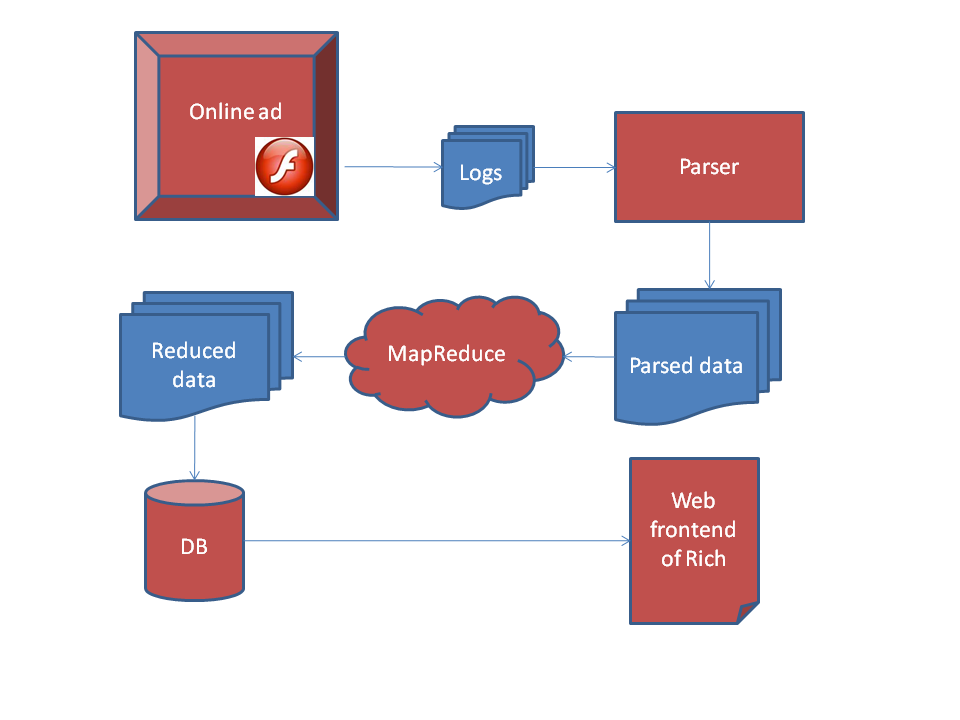
\includegraphics[scale=0.5]{gfx/general/System1.eps}
    \caption{The Rich system as designed today}
    \label{fig:rich}
\end{figure}
 
The flow of the system is visualized in figure \ref{fig:rich}, where the first step in this process is the execution of a script inside an Internet advertisement using Rich. This is usually a Flash ActionScript or JavaScript triggered to respond to various user events, such as clicks and mouse movements, as well as timed events like how long the user saw the advertisement. The script then sends the associated data to a central log server. The parser reads these logs at scheduled times and interprets the logged events into a session aggregated form. The parsed data are then transformed into the final presentation data using Hadoop, "a Java software framework that supports data-intensive distributed applications [...] inspired by Google's MapReduce"\footnote{http://wiki.apache.org/hadoop/ProjectDescription, May 20, 2010}. This readily calculated data is stored in a relational database in order to be accessible to an end user via a web application.

There are two reasons for doing all of this processing, rather than simply storing the logged user events directly in the database and perform calculations on the fly when requested from the web application:
\begin{itemize}
\item Storing individual user data is not only superfluous as this kind of data is never presented, it is also ethically unjustifiable.
\item According to the CTO at Burt, a single large global advertisementcampaign may be viewed in the order of $10^9$ times during a month. Calculating statistical properties of this data on the fly is simply not viable.
\end{itemize}

\section{Understanding the existing system} \label{sec:Understanding the existing system}
Today Rich arranges the gathered session data into two different piles; categories and metrics. For one tuple of data there are around 35 to 45 measurements. These measurements are divided as 20 to 30 "categories", and around 15 other measurements we will call "metrics". The differentiation of these two groups are just a simplification for Burt to handle the data, in the sense that questions upon the data are only made on the categories, whereas the metrics are simply interesting as output. What kind of measured value is considered a category or a metric is decided by a domain expert at Burt, since there is no inherent property of the data that puts it in either group. An example category is website, and an example metric is the number of times an advertisement has been clicked.

What is then performed is a MapReduce job (described in section \ref{subsec:MapReduce}), where the mapping is done on the tuples containing date, campaign id and a category, for each possible category. The reduction step aggregates the metrics in a non-trivial way, i.e. it is not simply an additive process, but the details are not of interest for the project. The result of the MapReduce is stored in accordance with a very minimalistic MySQL schema, with a column for date, campaign id, category name, value of the category and one column for each of the metrics.

\section{Initial problem statement} \label{sec:Initial problem statement}
Even with a system like the one described above, the management of data of this magnitude is a challenge. Due to this, Burt has currently limited the final presentation of the data to only include metrics that are highly relevant and relatively easy to calculate, as well as limiting themselves to only being able to specify, or fixate, at most one of the categories at a time. The problem is that agencies using Rich can not request information that is out of the ordinary. To make things worse, "the ordinary" is quite narrow. Hence our problem was to find a way of redesigning the highlighted sections of figure \ref{fig:rich_high} to allow for more complex questions to be answered by the data.

\begin{figure} [h]
    \centering
    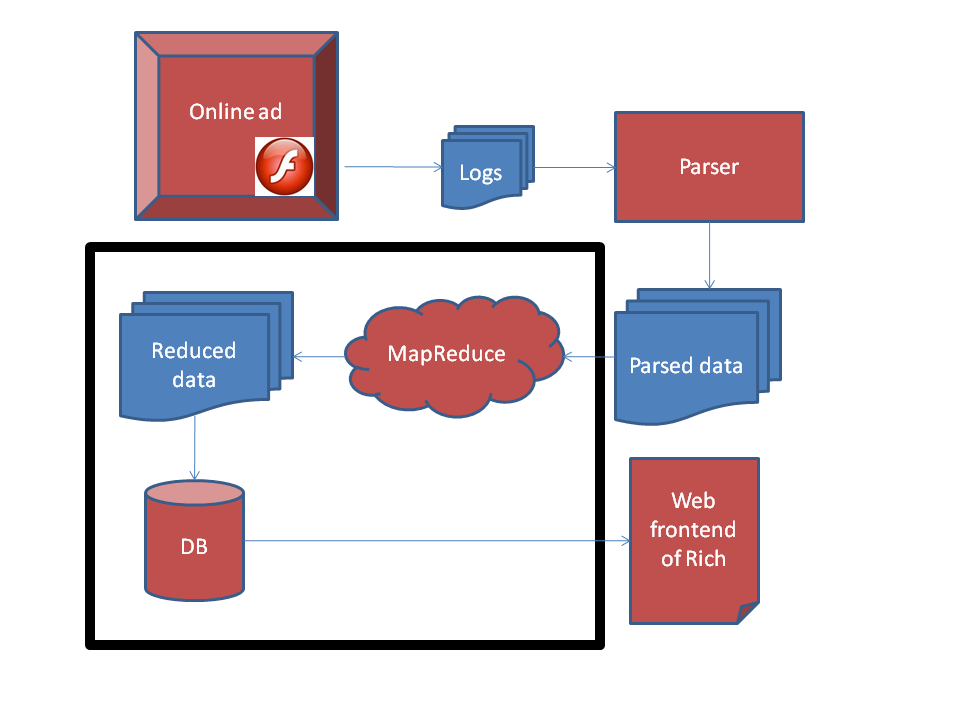
\includegraphics[scale=0.5]{gfx/general/System2.eps}
    \caption{The parts of the Rich system that we are to redesign}
    \label{fig:rich_high}
\end{figure}

The first delimitation we have to make is what kind of more complex questions do we want to be able to answer. This was relatively straightforward to determine since the request was to enable the querying of data where more than one category was specified and fixed. In other words, we want to ask a question where we specify a set of categories, and fix their values. This kind of question we will henceforth call a closed question. The second kind of query is where we ask for data where a set of categories are specified, and all but one of them are fixed. This kind of question we will henceforth call an open question. The number of categories in a question is by Burt called the drill-down depth.

Whatever changes suggested, or whatever system to use, they are still subject to the following criteria:
\begin{itemize}
\item Any query of the above described type should be able to be answered in real-time.
\item Insertion of data will be done once every 24 hours, and will be in the order of $10^9$ rows.
\item The system must be able to scale well horizontally (often also refered to as scale out, which means it should be possible to add more nodes to the system, i.e. more computers).
\end{itemize}

\pagebreak
\chapter{Concepts} \label{chap:Concepts}

\section{Storage solutions}

The term database is used to describe a variety of systems employed to organize storage of data. There are different types of systems as well as models that do this in different ways and here we try to examine the fundamental differences of the more prominent ones.

First, we will explain the general concepts of row- vs column-oriented storage, that can be applied in a variety of scenarios. Then we will cover the differences between the traditional relational database systems that have been around for several decades and some systems that have emerged from the recent NoSQL movement, reflecting renewed interest in non-relational storage models.

\subsection{Row-oriented}

A row oriented system concerns \textit{tuples} and \textit{attributes}. A tuple represents an object and an attribute represents one piece of information about an object. Usually, this is then thought of (or even stored as) a table where the tuples corresponds to rows and the attributes to columns.\cite{Codd} This is the primary way of thinking about data in the relational model and will be outlined further in section \ref{subsec:Relational models}.

\subsection{Column-oriented}

A column-oriented database is similar to a row-oriented, but as the name reveals it focuses on columns (attributes) rather than rows (tuples). A row-oriented database can easily operate on all the tuples in a system, while the column-oriented one is tuned to operate efficiently on a set of attributes for all tuples \cite{Copeland}.
\pagebreak
To make this clearer, consider this table of 1980's heavy metal songs:

\begin{table} [ht]
\caption{Table to illustrate column-oriented storage, as opposed to row-oriented}
\centering
\begin{tabular}{l|l|l|l}
\hline\hline
Title		            &	 Artist        &  Album           &  Year \\
\hline
Breaking the Law    &  Judas Priest  &  British Steel   &  1980 \\
Aces High           &  Iron Maiden   &  Powerslave      &  1984 \\
Kickstart My Heart  &  Motley Crue   &  Dr. Feelgood    &  1989 \\
Raining Blood       &  Slayer        &  Reign in Blood  &  1986 \\
I Wanna Be Somebody &  W.A.S.P.      &  W.A.S.P.        &  1984 \\
\hline
\end{tabular}
\end{table}

An example tuple is \textit{(Aces High, Iron Maiden, Powerslave, 1984)} and an example attribute is \textit{Album}.

In a row-oriented database this would be stored somewhat like this:

\begin{verbatim}
Breaking the Law
Judas Priest
British Steel
1980
Aces High
Iron Maiden
Powerslave
1984
Kickstart My Heart
Motley Crue
Dr. Feelgood
1989
Raining Blood
Slayer
Reign in Blood
1986
I Wanna Be Somebody
W.A.S.P.
W.A.S.P.
1984
\end{verbatim}

And in a column-oriented database:

\begin{verbatim}
Breaking the Law
Aces High
Kickstart My Heart
Raining Blood
I Wanna Be Somebody
Judas Priest
Iron Maiden
Motley Crue
Slayer
W.A.S.P.
British Steel
Powerslave
Dr. Feelgood
Reign in Blood
W.A.S.P.
1980
1984
1989
1986
1984
\end{verbatim}

Now, let us consider how 4 different database operations would perform in these two systems.

Creating a new tuple in the first case simple involves writing the new tuple to the end of the data. In the second case, this requires careful insertions at different places in the data.

Creating a new attribute reverses the situation. In the column-oriented case, data just has to be appended to the end, while it is non-trivial in the row-oriented case.

Fetching all songs from the year 1984 is easier in a row-oriented system than in a column-oriented one. For every tuple, we check if the fourth value is 1984 and if so we pull the whole tuple out. In the column-oriented system we have to scan the years and remember the indexes of all occurrences of 1984 and then scan though all the data and using the indexes to determine what to extract.

Getting the sum of all years is easiest in the column-oriented system since they are all found consecutively.

As a summary, we can conclude that row-oriented system are best when there is a need to create many new rows and retrieve many columns for the same row at the same time. On the contrary, column-oriented system are best when new columns have to be created often and there are aggregations performed over many rows, but few columns, at a time. In other words, the row-oriented systems are well suited for the class of systems referred to as OLTP (online transaction processing) where the system has to respond immediately to user requests. Column-oriented systems are a better match for OLAP (online analytical processing) which has to respond quickly to multidimensional analytical queries \cite{CoddCodd}.

\section{Relational model} \label{subsec:Relational models}

For the several decades the most common data storage model has been the relational model. The term was originally defined by Edgar Codd at IBM Almaden Research Center in 1970 \cite{Codd}. Software implementing this model is called a relational database management system, or RDBMS. The less strict term "relational database" is often used in its place.

A relation is defined as a set of tuples having the same attributes. Usually one of these tuples represents an object and its associated information. A set of one or more attributes has to be chosen as the primary key, which must be distinct among all tuples in the relation. The relation itself is usually described as a table where each tuple corresponds to a row and each attribute to a column. Both rows and columns are unordered. 

Relations can be modified using insert, delete and update operators. They can also be queried for data by operators to identify tuples, identify columns, combine relations and so on. The most common way to do this is by using the "structured query language", SQL.

Furthermore, two concepts of importance are the foreign keys and indexes. A foreign key is a reference to a tuple in a relation. Usually a different tuple in a different relation, but not necessarily so. Compared to primary keys, foreign keys need not be unique. This allows a single tuple to be referenced by any number of tuples.

Indexes, just like primary and foreign keys, are defined as a set of attributes on a relation. Querying a relation over the indexed set of attributes won't require the RDBMS to check each single tuple for a match, but rather use a precomputed index to find them quicker.

\section{NoSQL models}
Carlo Strozzi first used the term NoSQL in 1998 as a name for his open source relational database that did not offer a SQL interface\footnote{http://www.strozzi.it/cgi-bin/CSA/tw7/I/en\_US/nosql/Home\%20Page, Retrieved May 20, 2010}. The term was reintroduced in 2009 by Eric Evans in conjunction with an event discussing open source distributed databases\footnote{http://blog.sym-link.com/2009/05/12/nosql\_2009.html, Retrieved May 20, 2010}. This time it did not refer to a particular system, but rather a step away from the relational model altogether (as opposed to the query language). Appropriate or not, the name attempts to describe the increasing number of distributed non-relational databases that has emerged during the second half of the 2000's \cite{BigTable}\cite{Cassandra}.

Some general, but not ubiquitous, traits most of the NoSQL systems share:

\begin{itemize}
\item They lack fixed schemas
\item They avoid joins (the operation of combining relations)
\item They scale horizontally
\end{itemize}

Furthermore, they all satisfy very different needs. Some systems, like the document oriented ones, gain an immense ease-of-use, while most of the key-value or column oriented ones make it easier to distribute data over clusters of computers.

In order to fully understand the difference between all these systems and their trade-offs, Brewer's CAP theorem is of great help. It was first presented in a talk by Eric Brewer in 2000 and is based on his work and observations at UC Berkley. Seth Gilbert and Nancy Lynch provided a formalisation and a proof of the theorem two years later \cite{GilbertLynch}.

The theorem states that it is impossible for a web service to provide guarantees for \textit{Consistency}, \textit{Availability} and \textit{Partition Tolerance} at the same time. All three of these properties are desirable and are defined as follows:

\subsubsection{Consistency}

"There must exist a total order on all operations such that each operation looks as if it were completed in a single instant" \cite{GilbertLynch}. A service that is consistent operates fully or not at all. 

Traditional relational databases work with transaction semantics which provides this proparty; each work-unit performed must either complete fully or have no effect at all. This is usually refered to as one of ACID properties which states that a transaction must be atomic, consistent, isolated and durable.

\subsubsection{Availability}

"For a distributed system to be continuously available, every request received by a non-failing node in the system must result in a response" \cite{GilbertLynch}. Availability means exactly what it sounds like; the service is available and will respond to the messages it is being sent. Unfortunately it is a property that tends to desert you when you need it the most. Services go down at busy times just because they are busy.

\subsubsection{Partition Tolerance}

"In order to model partition tolerance, the network will be allowed to lose arbitrarily many messages sent from one node to another. When a network is partitioned, all messages sent from nodes in one component of the partition to nodes in another component are lost." \cite{GilbertLynch}

If the service server runs on a single machine it acts as a kind of atomic entity in that it either works or does not. If it has crashed it is not available, but it won't cause data inconsistencies either. Once the service gets distributed then there's a risk of partitions forming and the only way to handle these is to compromise on either consistency or availability.

\subsubsection{Dropping Partition Tolerance}

If you want to run without partitions you have to stop them happening. One way to do this is to put everything on one machine. There are, of course, significant scaling limits to this.

\subsubsection{Dropping Availability}

This could be seen as the opposite of dropping partition tolerance. On encountering a partition event, the service simply waits until data the nodes are back online. Implementing such a system in practice can be hard if everything is supposed to come back online gracefully.

\subsubsection{Dropping Consistency}

Accept that things will become "Eventually Consistent" \cite{Vogels}. Many inconsistencies don't actually require as much work as one might think. For example, if two orders are received for the last book that's in stock, there will be -1 book left, but this can simply become a back-order and the customer does not have to be affected by the inconsistency.

\subsection{Key-Value}

This class of storage systems arguably have the simplest data model. Rather than tables or semi structured documents, data is just organized as an associative array of entries. A unique key is used to identify a single entry and all of the three available operations use this key; delete the given key, change the entry associated with the key, insert a new key with associated data.

"It is basically just a big, distributed, persistent, fault-tolerant hash table."\footnote{http://project-voldemort.com, Retrieved May 20, 2010}

Noteworthy is that even though such a store is very straightforward to the application programmer, implementations often store data using a more traditional model behind the scenes. While the key-value-store looks and acts like an associative array, it may rely on tables, indexes and other artifacts of relational systems to be efficient in practice.

\subsection{Document-oriented}

Document-oriented databases are semi structured data storages, usually implemented without tables. The idea is to allow the client application to add and remove attributes to any single tuple without wasting space by creating empty fields for all other tuples. This means that all tuples can contain any number of fields, of any length. Even if used in a structured way, there are no constraints or schemas limiting the database to conform to a preset structure. This means that the application programmer gains ease of use and the possibility to create very dynamic data. The cost for all of this is the lack of a safety net and, to a certain degree, performance.

A document-oriented database can be implemented as a layer over a relational or object database. Another option is to implement it directly in a semi-structured file format, such as JSON, XML or YAML.

Traditional concepts like indexes and keys are often employed in the same sense as in relational databases. By using these, one is supposed to achieve almost the same performance as would be possible in a system implemented with tables.

\section{Data processing}

\subsection{MapReduce} \label{subsec:MapReduce}

MapReduce is a programming model supporting distributed computing on large data sets. It was first presented in the paper "MapReduce: Simplified Data Processing on Large Clusters" by the Google employees Jeffery Dean and Sanjey Ghemawat \cite{MapReduce}.

The user of a MapReduce framework provides two functions; a "map-function", which is meant to process a subset of the original problem and return the result as a list of (A,B)-tuples, and a "reduce-function", which given an A value and a list of B values produces a list of results that is the final answer for all A-parts. The signatures are also explained by the listing \ref{MapReduceSignatures}.

Both the map- and the reduce-function should be written purely functional (i.e. without side-effects), which is what allows them to be run in parallel. This allows them to be easily distributed over a cluster of nodes. Coordination by a master is then only required when grouping the outputs of the map-nodes together, before sending them off to the reduce-nodes. 

An example that creates an inverted index for a collection of documents can be found below in listings \ref{MapReduceMap} and \ref{MapReduceReduce}.

%\begin{verbatim} \label{MapReduceSignatures}
\begin{lstlisting}[language=Python,caption={Signatures for the map and reduce functions},captionpos=b, label={MapReduceSignatures}]
  map:    (subproblem) -> list(A, B)
  reduce: (A, list(B)) -> list(result)
\end{lstlisting}

\begin{lstlisting}[language=Python,caption={An example map function, in pseudo-code.},captionpos=b, label={MapReduceMap}]
 void map(String documentID, String documentContent):
  for each word w in documentContent:
    Emit(w, documentID);
\end{lstlisting}

\begin{lstlisting}[language=Python,caption={An example reduce function, in pseudo-code.},captionpos=b, label={MapReduceReduce}]
 void reduce(String word, List documentIDs):
  List sortedIDs = sort(documentIDs)
  List distinctSortedIDs = distinct(sortedIDs)
  Emit(word, distinctSortedIDs);
\end{lstlisting}

\pagebreak

\chapter{Problem theory}

\section{Pre-study: Data generation}
Before we try to find out how to store the data we need to make sure that it is plausible to produce that data. By this we mean that the data can be generated in reasonable time, and for this specific purpose that means in 24 hours, since that will be the time between each MapReduce job.

\subsection{The required data}
In Burt's current system each data row produced by the MapReduce job mentioned in section \ref{sec:Understanding the existing system} contains:
\begin{itemize}
\item Date
\item Advertisement ID
\item Campaign ID
\item Category
\item Value in category
\item Several metrics
\end{itemize}

Here the first five items were part of the key in the MapReduce job, whereas the metrics were the aggregated data. What we will need the MapReduce job to output in order to answer both open and closed questions is:

\begin{itemize}
\item Date
\item Advertisement ID
\item Campaign ID
\item Category 1
\item Value in category 1
\item Category 2
\item Value in category 2
\item ...
\item Category n
\item Value in category n
\item Several metrics
\end{itemize}

\noindent where n may vary depending on which depth of drill-down we are currently outputting. Also here all items except the metric items were a part of the key in MapReduce. If we let c be the number of possible categories, n be the number of categories you want in your MapReduce output, and v be the average number of distinct values for each category then we can calculate the number of output rows from the MapReduce job. First we will have to choose n of the c categories, which can be done in ${ c\choose n}$ different ways. Then we will, for each of those categories, choose all combinations of possible values. This can be done in approximately $v^n$ ways. In total there are then ${c\choose n} * v^n$ unique keys in the MapReduce job, each one creating one output row. Since the only variable we can change here is $n$, we can call this number $output_n$.

But this is only for a fixed value for n, and we are interested in all combinations of aggregations where n goes from 1 to a set number m, so the final equation for approximating the number of output rows from the Mapreduce job will be $output_{tot} = \displaystyle\sum\limits_{n=1}^m {c\choose n} * v^n$. 

\subsection{Partial MapReduce jobs}
If the reduction step in the MapReduce job were to be simple additive aggregations of the metrics, then there is a possibility for an optimization. Given that we have calculated all output rows $output_n$, then it is possible to calculate $output_{n-1}$ from $output_n$. This can be done by:
\begin{enumerate}
\item For each key of $n-1$ categories and their values you want to produce:
\item Choose an n$^{th}$ category that is not in the key.
\item Take all rows from $output_n$ that matches the key and also have the nth category, regardless of the values they have for that category.
\item Additively aggregate all the metrics for said rows, and put them as metrics for the key in step 1. 
\item output as a row in $output_{n-1}$.
\end{enumerate}

This realization made us investigate what kind of operations where performed in the current reduction step. Unfortunately there were several non-trivial, non-additive operations performed and so we had to dismiss this optimization. This led us to the conclusion that if MapReduce were to be used then it would need to produce the complete set of data rows that were to be stored, and not just a subset. Since the amount of computation that needs to be done to compute $output_{tot}$ is immense, we came to the conclusion that it is best that MapReduce is performed, and we can focus on storing the data.

\subsection{Time consumption}
How much time a MapReduce job takes is of course dependant on how many computers are used in the cluster, and their respective performance. So to say that a certain job may take at most 24 hours is not a valid constraint unless you also limit the available computing power. What we did was to implement our own MapReduce algorithm, and used that as well as the Hadoop MapReduce (described in section \ref{sec:Hadoop MapReduce}) to try and get an idea of the expected time consumption. Our tests suggested that it probably is not feasible to use an $n$ larger than 4. This made us question the necessity to actually perform the MapReduce job for all combinations of possible keys, or in other words; is every possible drill-down in the data really interesting, or is only a subset of them of importance?

\subsection{White-listing categories}
By defining a set of drill-downs that should be possible to perform we can greatly reduce the cost of the MapReduce job. This white-list is needed to be done on the keys of the mapping in the MapReduce step, but intuitively done only on a per-category basis, independent on the values of the categories. An example of such a white-list could look like (if the possible categories where Site, Country, Placement and Adload):
\begin{itemize}
\item Site
\subitem Country
\subsubitem Adload
\subitem Adload
\item Adload
\subitem Placement
\subitem Country
\item Placement
\item Country
\end{itemize}

This would create the following tuples of categories for the MapReduce job to produce: (Site), (Adload), (Country), (Placement), (Site, Country), (Site, Adload), (Adload, Country), (Adload, Placement), (Site, Country, Adload). Keep in mind that the order in these tuples does not matter, so the tuple (Site, Country, Adload) is equivalent to the tuple (Adload, Country, Site). If we denote the total number of tuples of size $m$ for $d_m$, and then assume that the number of potential interesting drill-downs is limited, then we can change the cost of the MapReduce job from $\displaystyle\sum\limits_{n=1}^m {c\choose n} * v^n$ to $\displaystyle\sum\limits_{n=1}^m d_n * v^n$. This is a significant improvement if $d_m$ is not immense for each value of m.

\subsection{Automating the white-list}
But how would one decide what drill-downs to put down on the white-list? A domain expert can try to produce a draft of the list, but in the end it will be the customers that decide what statistics they are actually interested in. For this purpose it could be interesting to be able to change this white-list programmatically, as a reaction to a customer's action on the website. For example:
\begin{itemize}
\item There could be an interface where paying customers can request drill-downs that do not exist at present.
\item It could be that all drill-downs seem available to the customer, but once he tries an attempt to access one that is not computed a request is sent automatically.
\end{itemize}

\section{Properties of the data} \label{sec:Properties of the data}
A noteworthy property of the data rows that are output by the MapReduce job is that they are completely independent of any other data rows. What this means is that for any arbitrary data row in the output, that data row does not require the existence of any other form of data in order to convey all of its information. The data is both self describing, and independent.

This observation simplifies the problem immensely, in the sense that scaling the data horizontally is no longer a problem. This can for example be done by spreading the data randomly across an arbitrary number of nodes. When a query is being processed, it is sent to each node, and then the final result is gained by taking the union of each node's result. This kind design is possible independent of database system, and therefore will simplify both the designs of the systems being produced, and the testing to be performed.

\pagebreak
\chapter{Implementations}
In this chapter we will discuss different implementations of database storage systems. The systems that qualified for testing will each be presented in some detail, but we will also mention several systems that we did not test. We try here to focus on describing the systems both to give an understanding of their design, but also their reliability, and the exact way in which we used them in order to make our tests reproducible. We will also discuss the MapReduce implementation currently used by Burt, Hadoop.
\section{Database management systems}
When deciding upon which systems to test we first needed to specify on what criteria we should base our decision. We want each system to be tested to be stable, that means no alpha-staged software, and the system should have been in use of at least one large commercial application. We want to test systems from all aspects of the CAP theorem, that is CA-systems, CP-systems and AP-systems. We should try to limit our selection to fit the required time we have at our disposal, in other words, we should not try out two systems that are too similar, instead focus on finding differences in the set of possible systems. We are also only interested in systems that conform to one of the paradigms described in chapter \ref{chap:Concepts}, since our data is best modelled in those ways. In table \ref{table:allsystems} we can find all systems that we considered as candidates for testing, and in figure \ref{fig:cap} we see the five systems that where chosen among these candidates.

\begin{table} [ht]
\caption{The list of possible candidate systems}
\centering
\begin{tabular}{l|l|l|l}
\hline\hline
Name		          &	Design          & CAP         & Comment                          \\
    		          &	Paradigm        &             &                                  \\
\hline
CouchDB           & Document        & AP          & Similar to MongoDB.              \\ 
MongoDB           & Document        & CP          & Chosen.                          \\
Neo4j             & Graph           & unknown     & Our data is not naturally        \\ 
                  &                 &             & representable as a graph.        \\
HBase             & Column          & CP          & Chosen.                          \\    
Memcachedb        & Key-Value       & unknown     & Stores data in                   \\ 
                  &                 &             & memory, inapplicable.            \\         
Riak              & Key-Value       & CP          & Similar to Cassandra.            \\
Project Voldemort & Key-Value       & AP          & Chosen.                          \\         
Redis             & Key-Value       & CP          & Stores data in                   \\ 
                  &                 &             & memory, inapplicable.            \\         
SimpleDB          & Key-Value       & AP          & Only available through           \\ 
                  &                 &             & Amazon.                          \\     
Cassandra         & Column          & AP          & Chosen.                          \\         
Hypertable        & Column          & unknown     & Similar to HBase.                \\     
Db4o              &                 & unknown     & Not open-source for              \\
                  &                 &             & commercial use.                  \\ 
Mnesia            & Relational      & AP          & Restricted to the Erlang         \\ 
                  &                 &             & programming Language.            \\        
MySQL             & Relational      & CA          & Chosen.                          \\
Mondrian          & OLAP            & unknown     & Wrong design paradigm.           \\
\hline
\end{tabular}
\label{table:allsystems}
\end{table}

\begin{figure}
    \centering
    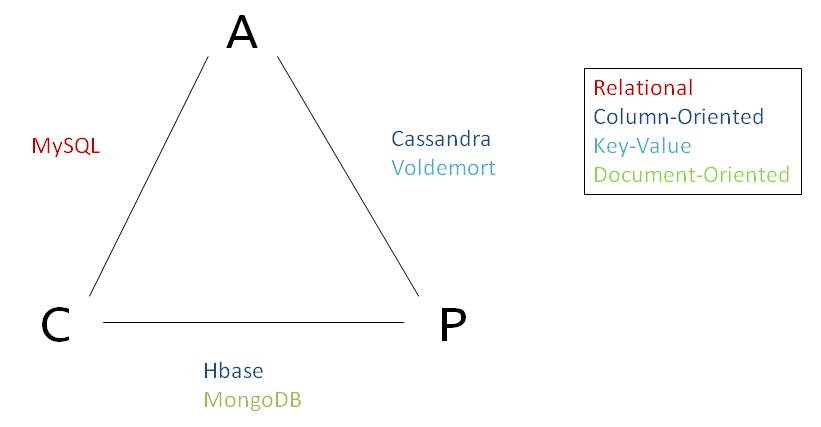
\includegraphics[scale=0.5]{gfx/general/CAP.eps}
    \caption{The CAP-theorem and the investigated systems relations to it}
    \label{fig:cap}
\end{figure}

\subsection{Cassandra}
Cassandra is an Apache Software Foundation project \cite{Cassandra}. It is a distributed database management system based around a column-oriented architecture. It was initially developed by Facebook to be a hybrid between Google's BigTable \cite{BigTable} and Amazon's Dynamo system \cite{Dynamo}. At its core it is a four to five dimensional key-value store with eventual consistency. You can choose to model it as:
\begin{itemize}
\item Keyspace $->$ Column Family $->$ Row $->$ Column $->$ Value
\item Keyspace $->$ Super Column Family $->$ Row $->$ Super Column $->$ Column $->$ Value
\end{itemize}
We choose to work with Cassandra Version 0.6 Beta, using a Thrift gateway \cite{Thrift}.
\subsection{HBase}
HBase is a database developed as a part of the Hadoop project by Apache's Software Foundation. It can basically be seen as the Hadoop database, and it runs on top of the Hadoop Distributed File System (HDFS). HBase is a column oriented database modeled after Google's BigTable design. HBase tables can be used as both the input and output for MapReduce jobs run in Hadoop. HBase can be accessed through a Java API, and also through a REST and Thrift gateway.

The data model of HBase is most easily seen as a four dimensional dictionary. The keys of this dictionary then are, in order: Table, Row, Column, Time-stamp, which then point to a value.

Our use of HBase utilized the Thrift gateway, and we used HBase Version 0.20.3.
\subsection{MongoDB}
MongoDB is a scalable, high-performance, open source, document-oriented database. Development started in October 2007, and it is still a active project. MongoDB stores its data in binary JSON-style documents, and is mainly used for problems without strong transactional requirements. Like other document oriented databases it is schema-free, easy to set up and use, and easy to scale out on different servers.

The version of MongoDB that we have used for our tests is the Linux 64bit 1.4.2 version. We are accessing MongoDB through the ruby gems Mongo API.
\subsection{Voldemort DB}
Voldemort is a distributed eventually consistent key-value storage system developed by LinkedIn. It is supported by a MySQL or Berkley DB back-end, and what Voldemort DB provides for you is an easy way to distribute, replicate, version, and partition your data. Each node is independent of other nodes with no central point of failure or coordination, and it has a good single node performance.

The data model for Voldemort is extremely straightforward, since it is used as a simple key-value store with strings for both keys and values. It also provides libraries for serialization of lists and tuples with named fields.

We choose to try this storage engine version 0.80 using the Berkley DB back-end and we use the included ruby API to access the system.
\subsection{MySQL}
MySQL is a well known relational database management system first released in 1995. It is typically used in small to medium scale single-server deployments. But on larger scales multiple-server MySQL deployments can be used, and the most common ways to do so is to use full replication to increase read capacity or sharding to increase write capacity. What distinguishes MySQL from some other relational DBMS systems are that it supports multiple storage engines, both native, partner developed and community developed.

We used MySQL version 14.14 distribution 5.1.37 with the MyISAM engine, and used the ruby gems MySQL API to communicate with the system.
\section{Hadoop MapReduce} \label{sec:Hadoop MapReduce}
Hadoop is an Apache project that develops open source software for distributed computing. One of their sub-projects is Hadoop MapReduce which is a  programming model and software framework for writing applications that rapidly process vast amounts of data in parallel on large clusters of compute nodes\footnote{http://hadoop.apache.org/mapreduce/, 21 May, 2010}. This is the implementation of MapReduce that Burt are currently using, and is the one that will be used for future work as well.

\pagebreak

\chapter{Designs}
In this chapter we will look at the different designs we used for the systems. But before trying to come up with designs for the different database systems, we must look at the problem, and the data, to see what designs might be satisfying, and best model the data and information.
\section{Requirements on the design}
So how do we deem a design as satisfying? The requirements from Burt described in section \ref{sec:Initial problem statement} must hold. Two of those requirements, real-time querying of the data and horizontal scalability, are things we can guarantee at the design level, whereas insertion time is what we will need to measure in our tests. To guarantee real-time querying we will use different ideas of indexing, and to guarantee horizontal scalability we will either obtain it as an inherent property of the system, or by making sure that we do not remove the quality of independence of the data described in section \ref{sec:Properties of the data}.
\section{Closed queries} \label{sec:Closed queries}
If we start by creating a design able to answer the closed questions only, then this can be done relatively straightforwardly. Given an output data row from the MapReduce job we can form a string describing the categories and their values. To create this string we simply concatenate the categories and their respective values using a delimiter. For simplicity we will call this string a category-string. If we then store this category-string together with the metrics using an index on the category-string, anyone wanting to ask a closed question can then create the category-string, and search the index.
\section{Open queries} \label{sec:Open queries}
A row in the output data in the MapReduce job has a certain number of categories, lets call this number $c$. This row is then a part of the result of a total of $c$ open queries, one for each category you allow to be unspecified. This means that for a data row which has the categories and values:
\begin{itemize}
\item Category: Site, Value: www.awebpage.com
\item Category: Country, Value: Swe
\item Category: Adload, Value: 5
\end{itemize}

Then all the open queries that this row would be in the results of are (using the pipe symbol as the delimiter in a category-string notation):
\begin{itemize}
\item $"Site|www.awebpage.com|Country|Swe|Adload|"$
\item $"Site|www.awebpage.com|Country||Adload|5"$
\item $"Site||Country|Swe|Adload|5"$
\end{itemize}

If we express one of these in natural language, the second one would read: Get all rows of drill-down depth 3 where the categories are Site, Country and Adload, where the Site is www.awebpage.com and Adload is 5. Country can be any value.

We here suggest a couple of different designs that will be able to handle real-time querying of this kind of representation. The category-strings of closed queries and open queries are sometimes refered to as "full keys" and "partial keys" respectively. 
\subsection{Duplication of input}
In this design we create $c$ duplicates of each data row, and for each category-string produced we exclude one of the category values, as in the example above. The category-string is stored together with the excluded category value and metrics, with an index on the category-string.

This design we use for one MySQL system.
\subsection{Multiple indexes}
In this design we create $c$ category-strings where we exclude one of the category values, as in the example above. The category-strings are stored together with the closed category-string and metrics, with an separate index on each of the category-strings.

This design we use for one MySQL system.
\subsection{Inverted indexes} \label{subsec:Inverted indexes}
This design is a space optimization of the Duplication of input design, where we divide the data in two different tables, one for the metrics (metrics table), and one for the category-strings (questions table). Each data row from the MapReduce job creates one row in the metrics table, containing the metric values and the closed category-string, as well as a unique identifier. Each data row also creates $c$ entries in the questions table, one for each possible open category-string, where the questions table basically works like a dictionary mapping the category-strings to the unique identifiers in the metrics table. The metrics table uses an index on the unique identifier, and the questions table uses an index on the category-string.

This design we use for two MySQL systems, two Cassandra systems, one HBase system, two MongoDB systems and one Voldemort DB system.
\section{Indexing on strings}
In all of these designs we index upon strings, which can become a performance issue, since those indexes can become rather large. A category-string with up to six categories can be well over 80 characters long, and creating an index with 80 bytes can be difficult to do efficiently. To handle this problem we propose a 4-byte hashing of the string. This means that instead of storing just the string, with the index on the string, you store both the string and a 4-byte hashing of the string, and then index upon the hash value instead. When searching for a particular string you then hash the string again, look up all hash values matching the hash using the index, then do a secondary search on the result set finding only the rows matching the exact string. We chose a 4-byte hashing because it prooved to be efficient enough, creating on average of 0.0002 hash collisions per hash value for our data\footnote{This was tested on a generated set of 1409919 distinct queries, yielding 1409625 different hash values.}.

We used this technique on 3 MySQL systems, one Voldemort DB system and one MongoDB system.

The hashing method we use is the Jenkins hash function \cite{Jenkins}.
\pagebreak

\chapter{Method}
\section{Precondition}
Hadoop produces data that describes all the data Rich can present to the end-user. These data entries are organized in files with one entry per row. Every entry, and hence every row in the file, contains three parts; a campaign id, a set of category values and a set of metrics. An important property of this data is that the union of the campaign id and the category values works as a key that will be different for each row ever produced by Hadoop. The exact syntax of these data rows is up to the user implementing the Hadoop script and should be laid out in a way that is convenient for that data storage solution. Being able to import this data quickly is an important property of any system, since this puts an upper bound on how much data it can store over time.

\section{Postcondition} \label{sec:Postcondition}
After the data has been stored Burt must be able to retrieve metrics using two methods. The first one is to query the storage system with a full key (a campaign id and a set of category values) and have it return the corresponding metrics, if any. The second one is to supply a partial key, which is the same as a full key, except that for one of the categories, only the category name is supplied and its value is left unspecified. In this case any value from the same category will match the one left unspecified and the system should return all matching entries, which could be any number from 0 and up. No queries will contain two or more unspecified categories, even if such a generalization could be made quite easily in most implementations. Both of these two retrieval methods must be able to perform their tasks in less than a second, for any amount of data that Burt would ever be able to store.

In our study we are interested in comparing how well a set of candidate storage systems would perform these tasks. This has been split up into three stages:

\begin{description}
\item[Stage 1, Culling] In the first part we're simply interested in culling the systems that cannot store data fast enough to be useful in practice. This will be done with relatively small data sets and only on a local machine.
\item[Stage 2, Comparison] In the comparison step the systems that passed the culling test will be run in a production environment and with more realistic data sets.
\item[Stage 3, Scaling] Finally, the system with the best performance in the comparison step will be run with an even bigger set of input data in order to verify that it scales as well as anticipated.
\end{description}
Apart from being run in different environments and on data of different sizes, every single test in every stage will be performed in the same fashion:

\begin{itemize}
\item A script will initialize the data storage by setting up the desired configuration, starting a server and making sure that the system doesn't contain any data all.
\item A data set of the desired size and syntax is deterministically generated and stored in files as if Hadoop had produced them.
\item The files are inserted into the storage system one by one. How this is done differs between the systems, but all of them measure the time it takes to perform this operation.
\item After every insertion a fixed number of queries is made on the data that have been inserted so far. Half of them are closed questions and the other half are open questions. The elapsed execution time of these operations are measured, and contingent behaviour and errors are caught and reported. A fixed percentage of the measured values (on the low and high ends of the scale) are discarded before any averages are computed, in order to get closer to the actual average, and avoiding the measurement of initial connection establishing etc.
\item When all data has been inserted, measurement averages are collected in a file and presented as plots of execution time as a function of data size. Two graphs are created after each test, one for insertion and one for querying. The insertion graph displays insertion time for one million rows in seconds against the number of rows in the database. The querying graph displays the average time in milliseconds against the number of rows in the database. This graph distinguishes between open and closed question.
\end{itemize}

The above steps are implemented as scripts for all systems in the test in order to be reproducible in detail. As much as possible of these scripts are implemented in a generic fashion so that only necessary parts will differ between the different systems. This ensures that they all handle the same data, use the same timing routines and produces the same kind of output.

\section{Delimitations}
None of the test stages were performed using distinct clients and servers; they are always run within a single computer. No actual distribution is taking place during the tests.

\section{Testing environment}
The tests were performed on two different environments. The culling stage were executed on one environment, and the comparison and scaling stages on a second. The motivation for such a separation is basically for the sake of simplicity. During the culling stage the tests were performed on a standard-model laptop computer, which is sufficient since what we mostly want to detect here if any system is orders of magnitude worse in comparison to the others. The comparison and scaling stages were performed on a much more rigorous platform, an instance in the Amazon S3 cloud. Once a test is initiated no other task is performed on the system.

\begin{table} [ht]
\caption{Hardware specifications for the test platforms}
\centering
\begin{tabular}{l|l|l}
\hline\hline
Spec     &  Laptop                  &  Amazon EC2 (Large Instance)  \\
\hline
CPU      &  XPS M1330 CORE 2 DUO    &  2 Intel(R) Xeon(R) CPU       \\ 
         &  T9300 2.50GHz           &  E5430 @ 2.66GHz              \\  
Ram      &  4,0 GB                  &  7,5 GB                       \\                
HDD      &  500 GB                  &  1000 GB                      \\  
\hline
\end{tabular}
\end{table}

\chapter{Tests}
\section{The culling stage}
\subsection{Experiments}
We will here present measurements of the stage 1 tests mentioned in section \ref{sec:Postcondition}. We produced two graphs for each system and configuration. The first graph plots average insertion time per row against the number of rows in the database. The second graph plots average querying time of both open and closed questions (as described in section \ref{sec:Initial problem statement}) against the number of rows in the database.

\begin{figure}
    \centering
    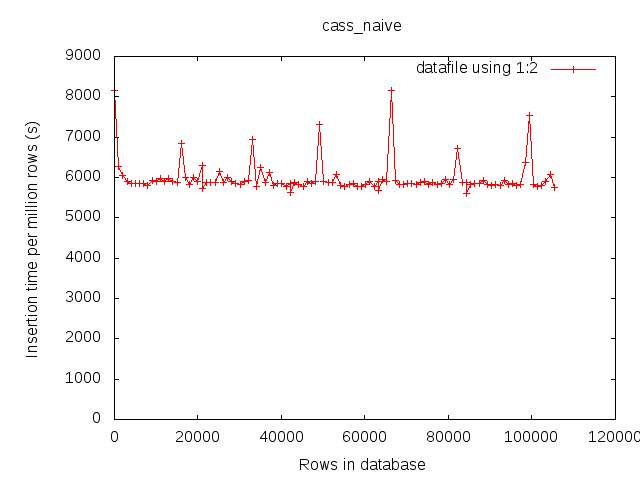
\includegraphics[scale=0.5]{gfx/stage1/cass_naive_insert.eps}
    \caption{Insertion in Cassandra, inverted indexing}
\end{figure}
\begin{figure}
    \centering
    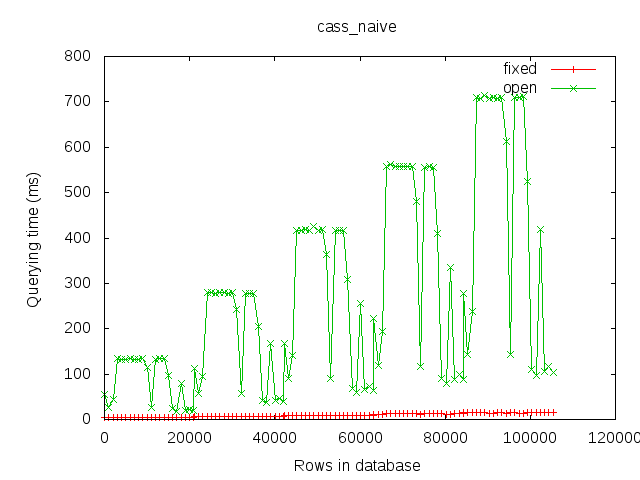
\includegraphics[scale=0.5]{gfx/stage1/cass_naive_query.eps}
    \caption{Querying in Cassandra, inverted indexing}
\end{figure}
\clearpage

\begin{figure}
    \centering
    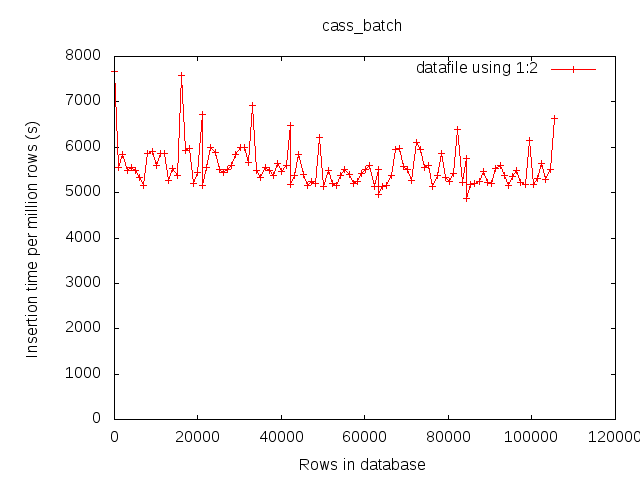
\includegraphics[scale=0.5]{gfx/stage1/cass_batch_insert.eps}
    \caption{Insertion in Cassandra, inverted indexing, batch insertion}
\end{figure}\begin{figure}
    \centering
    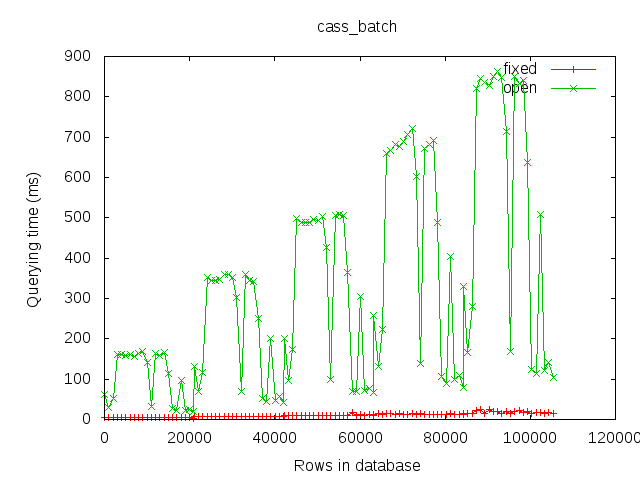
\includegraphics[scale=0.5]{gfx/stage1/cass_batch_query.eps}
    \caption{Querying in Cassandra, inverted indexing, batch insertion}
\end{figure}
\clearpage

\begin{figure}
    \centering
    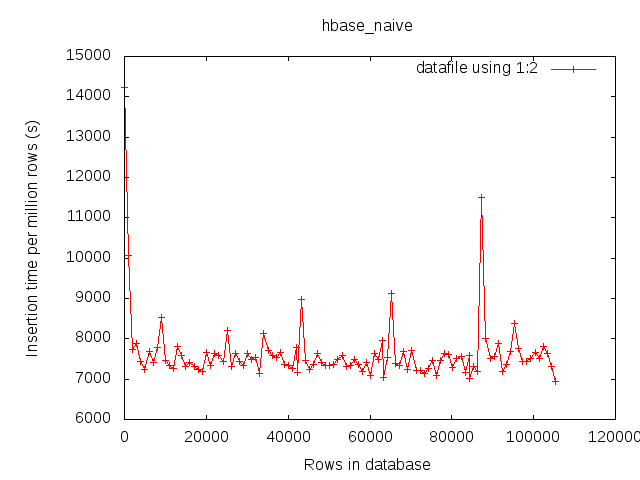
\includegraphics[scale=0.5]{gfx/stage1/hbase_naive_insert.eps}
    \caption{Insertion in HBase, inverted indexing}
\end{figure}
\begin{figure}
    \centering
    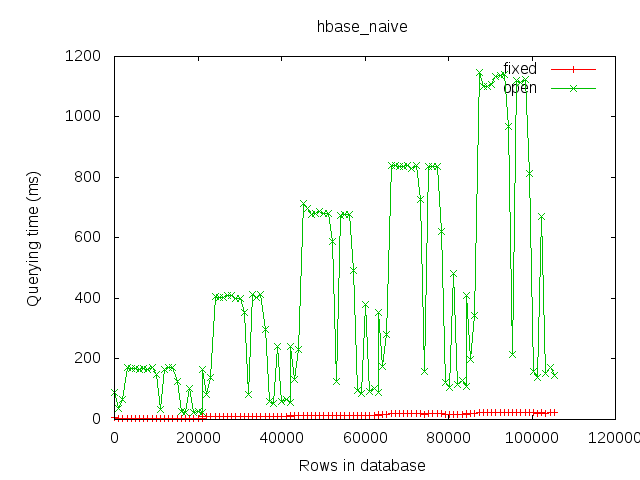
\includegraphics[scale=0.5]{gfx/stage1/hbase_naive_query.eps}
    \caption{Querying in HBase, inverted indexing}
\end{figure}
\clearpage

\begin{figure}
    \centering
    \includegraphics[scale=0.5]{gfx/stage1/mongo_inverted_index_insert.eps}
    \caption{Insertion in MongoDB, inverted indexing, string hashing}
\end{figure}
\begin{figure}
    \centering
    \includegraphics[scale=0.5]{gfx/stage1/mongo_inverted_index_query.eps}
    \caption{Querying in MongoDB, inverted indexing, string hashing}
\end{figure}
\clearpage

\begin{figure}
    \centering
    \includegraphics[scale=0.5]{gfx/stage1/mongo_inverted_index_nohash_insert.eps}
    \caption{Insertion in MongoDB, inverted indexing}
\end{figure}
\begin{figure}
    \centering
    \includegraphics[scale=0.5]{gfx/stage1/mongo_inverted_index_nohash_query.eps}
    \caption{Querying in MongoDB, inverted indexing}
\end{figure}
\clearpage

\begin{figure}
    \centering
    \includegraphics[scale=0.5]{gfx/stage1/mysql_dupe_insert.eps}
    \caption{Insertion in MySQL, duplication, string hashing}
\end{figure}
\begin{figure}
    \centering
    \includegraphics[scale=0.5]{gfx/stage1/mysql_dupe_query.eps}
    \caption{Querying in MySQL, duplication, string hashing}
\end{figure}
\clearpage

\begin{figure}
    \centering
    \includegraphics[scale=0.5]{gfx/stage1/mysql_inverted_index_insert.eps}
    \caption{Insertion in MySQL, inverted indexing, string hashing}
\end{figure}
\begin{figure}
    \centering
    \includegraphics[scale=0.5]{gfx/stage1/mysql_inverted_index_query.eps}
    \caption{Querying in MySQL, inverted indexing, string hashing}
\end{figure}
\clearpage

\begin{figure}
    \centering
    \includegraphics[scale=0.5]{gfx/stage1/mysql_inverted_index_nohash_insert.eps}
    \caption{Insertion in MySQL, inverted indexing}
\end{figure}
\begin{figure}
    \centering
    \includegraphics[scale=0.5]{gfx/stage1/mysql_inverted_index_nohash_query.eps}
    \caption{Querying in MySQL, inverted indexing}
\end{figure}
\clearpage

\begin{figure}
    \centering
    \includegraphics[scale=0.5]{gfx/stage1/mysql_multiple_hash_insert.eps}
    \caption{Insertion in MySQL, multiple indexes, string hashing}
\end{figure}
\begin{figure}
    \centering
    \includegraphics[scale=0.5]{gfx/stage1/mysql_multiple_hash_query.eps}
    \caption{Querying in MySQL, multiple indexes, string hashing}
\end{figure}
\clearpage

\begin{figure}
    \centering
    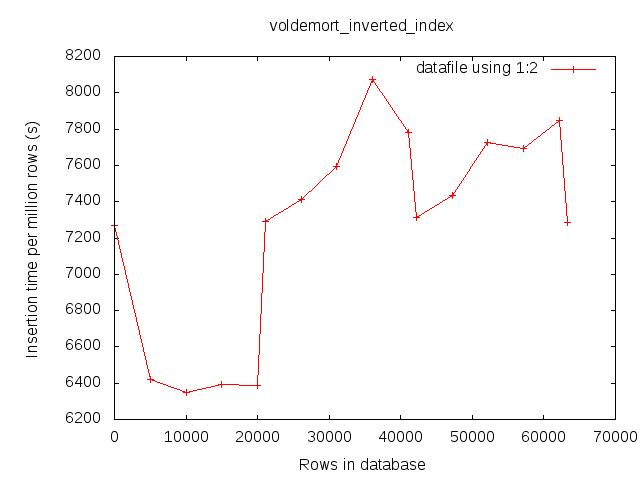
\includegraphics[scale=0.5]{gfx/stage1/voldemort_inverted_index_insert.eps}
    \caption{Insertion in Voldemort DB, inverted indexing, string hashing}
\end{figure}
\begin{figure}
    \centering
    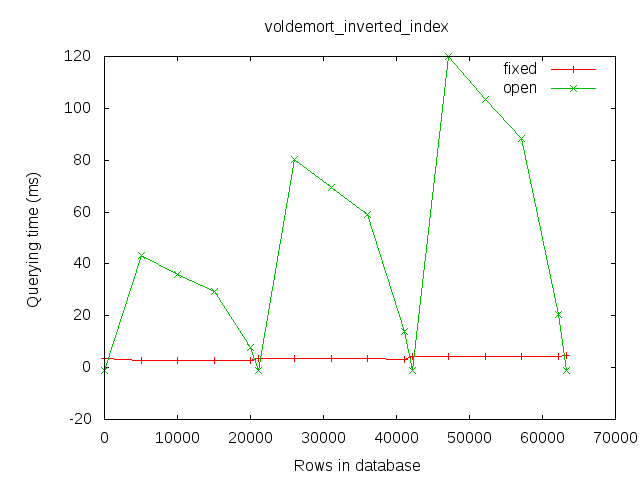
\includegraphics[scale=0.5]{gfx/stage1/voldemort_inverted_index_query.eps}
    \caption{Querying in Voldemort DB, inverted indexing, string hashing}
\end{figure}
\clearpage

\subsection{Analysis}

\begin{table}
\caption{Table of range of insertion times and querying times from stage 1}
\centering
\begin{tabular}{l|l|l|c|c}
\hline\hline
System              & Design            & Indexing on     & Insertion      &  Querying        \\
                    &                   &                 & time (s)       & time (ms)        \\
\hline
Cassandra           &  Inverted indexes & String hashing  & 5800-10400     & 10-780           \\
Cassandra (Batch)   &  Inverted indexes & String hashing  & 4750-7250      & 10-780           \\
HBase               &  Inverted indexes & String hashing  & 7200-14200     & 10-1160          \\
MongoDB             &  Inverted indexes & String hashing  & 220-480        & 2-8              \\
MongoDB             &  Inverted indexes & String indexing & 225-243        & 2-7              \\
MySQL               &  Duplication      & String hashing  & 15-45          & 1.5-4.5          \\
MySQL               &  Inverted indexes & String hashing  & 27-42          & 0.4-1.3          \\
MySQL               &  Inverted indexes & String indexing & 30-110         & 0.5-1.3          \\
MySQL               &  Multiple indexes & String hashing  & 10-47          & 0.4-1            \\
Voldemort DB        &  Inverted indexes & String hashing  & 6400-8100      & 5-120            \\
\hline
\end{tabular}
\end{table}

What is quite clear from the tests done at stage 1 is that we can divide the systems into two groups, with basically different orders of magnitude of performance. The slower group consists of Cassandra, HBase and Voldemort DB, and the other group consists of MongoDB and MySQL. In rough terms we can say that there is approximately a factor 100 in the difference of both input and querying time between these groups. Since this stage of the testing is to sort out systems that are highly likely not to be the best system, we will hereby discard all the systems in the slower group when performing the tests in stage 2. If both of MySQL and MongoDB proves to be performing on the same order of magnitude at later stages of testing, when testing on larger sets of data we might choose to revise this decision.

\section{The comparison stage}

\subsection{Experiments}
We will here present measurements of the stage 2 tests mentioned in section \ref{sec:Postcondition}. We produced two graphs for each system and configuration. The first graph plots average insertion time per row against the number of rows in the database. The second graph plots average querying time of both open and closed questions (as described in section \ref{sec:Initial problem statement}) against the number of rows in the database. In this stage we insert approximately 7.5 million rows into each system.

\begin{figure}
    \centering
    \includegraphics[scale=0.5]{gfx/stage2/mongo_inverted_index_insert.eps}
    \caption{Insertion in MongoDB, inverted indexing, string hashing}
    \label{fig:mongo_iii}
\end{figure}
\begin{figure} 
    \centering
    \includegraphics[scale=0.5]{gfx/stage2/mongo_inverted_index_query.eps}
    \caption{Querying in MongoDB, inverted indexing, string hashing}
    \label{fig:mongo_iiq}
\end{figure}
\clearpage

\begin{figure} 
    \centering
    \includegraphics[scale=0.5]{gfx/stage2/mongo_inverted_index_nohash_insert.eps}
    \caption{Insertion in MongoDB, inverted indexing}
    \label{fig:mongo_iini}
\end{figure}
\begin{figure} 
    \centering
    \includegraphics[scale=0.5]{gfx/stage2/mongo_inverted_index_nohash_query.eps}
    \caption{Querying in MongoDB, inverted indexing}
    \label{fig:mongo_iinq}
\end{figure}
\clearpage

\begin{figure} 
    \centering
    \includegraphics[scale=0.5]{gfx/stage2/mysql_dupe_insert.eps}
    \caption{Insertion in MySQL, duplication, string hashing}
    \label{fig:mysql_di}
\end{figure}
\begin{figure} 
    \centering
    \includegraphics[scale=0.5]{gfx/stage2/mysql_dupe_query.eps}
    \caption{Querying in MySQL, duplication, string hashing}
    \label{fig:mysql_dq}
\end{figure}
\clearpage

\begin{figure} 
    \centering
    \includegraphics[scale=0.5]{gfx/stage2/mysql_inverted_index_insert.eps}
    \caption{Insertion in MySQL, inverted indexing, string hashing}
    \label{fig:mysql_iii}
\end{figure}
\begin{figure} 
    \centering
    \includegraphics[scale=0.5]{gfx/stage2/mysql_inverted_index_query.eps}
    \caption{Querying in MySQL, inverted indexing, string hashing}
    \label{fig:mysql_iiq}
\end{figure}
\clearpage

\begin{figure} 
    \centering
    \includegraphics[scale=0.5]{gfx/stage2/mysql_inverted_index_nohash_insert.eps}
    \caption{Insertion in MySQL, inverted indexing}
    \label{fig:mysql_iini}
\end{figure}
\begin{figure} 
    \centering
    \includegraphics[scale=0.5]{gfx/stage2/mysql_inverted_index_nohash_query.eps}
    \caption{Querying in MySQL, inverted indexing}
    \label{fig:mysql_iinq}
\end{figure}
\clearpage

\begin{figure} 
    \centering
    \includegraphics[scale=0.5]{gfx/stage2/mysql_multiple_hash_insert.eps}
    \caption{Insertion in MySQL, multiple indexes, string hashing}
    \label{fig:mysql_mhi}
\end{figure}
\begin{figure}
    \centering
    \includegraphics[scale=0.5]{gfx/stage2/mysql_multiple_hash_query.eps}
    \caption{Querying in MySQL, multiple indexes, string hashing}
    \label{fig:mysql_mhq}
\end{figure}
\clearpage

\subsection{Analysis}
\begin{table}
\caption{Table of insertion times and range of querying times from stage 2}
\centering
\begin{tabular}{l|l|l|c|c}
\hline\hline
System       & Design            & Indexing on     & Insertion  &  Querying \\
             &                   &                 & time (s)   & time (ms)  \\
\hline
MongoDB      &  Inverted indexes & String hashing  & 12500      & 10-45     \\
MongoDB      &  Inverted indexes & String indexing & 2200       & 10-65     \\
MySQL        &  Duplication      & String hashing  & 1600       & 0.5-0.8   \\
MySQL        &  Inverted indexes & String hashing  & 1600       & 1-8       \\
MySQL        &  Inverted indexes & String indexing & 450        & 1-7       \\
MySQL        &  Multiple indexes & String hashing  & 2000       & 1-4.5     \\
\hline
\end{tabular}
\end{table}
The results from stage 2 give some interesting insights in the behaviour of the different solutions. From figure \ref{fig:mongo_iii} we can see that the Mongo DB solution that used our string hashing basically gave up at around 45 million rows, with a huge input time of 12500 seconds per one million rows. All the other systems succeded in inserting the targeted 70 million rows. The Mongo DB solution that did not use our string hashing fared better, with a seemingly logarithmic or linear growth peaking at 2200 seconds per one million rows in insertion time as seen in figure \ref{fig:mongo_iini}.

The almost periodical apperance of the graph in figure \ref{fig:mysql_iini} can be explained by the fact that the data inserted is simulated for ten days of data, where each day's batch starts of with the lowest number of categories, and then increases. This makes the category-strings mentioned in section \ref{sec:Closed queries} small in the beginning, making the indexing periodically faster. 

In terms of querying times not much needs to be said as all systems perform well. The only thing notably interesting is that the duplication design yields by far the fastest querying, always performing below one millisecond.

The curve of the duplication of input design used by the MySQL database in figure \ref{fig:mysql_di} is extremely interesting. It has one of the the best insertion times when there are below 30 million rows inserted, around 80 seconds per one million rows. After 30 million rows the insertion time increases dramatically, ending up approximately 20 times worse in an almost exponential fashion. This behaviour, signified by a first slow logarithmic growth, then turning into a rapidly growing curve can be seen in all four systems using our hashing design. With this kind of behaviour none of these systems will be usable for large quantities of data. The other two systems, who index on strings, have a much more linear growth throughout the tests, but the MySQL version is without a doubt faster, approximately 5 times.

\section{Extending the comparison stage}
So why did the four systems using our string hashing fail? From a purely theoretical point of view they should have a logarithmic growth at worst. Is this a problem rising from the hardware? Is it somehow related to the testing server residing in the cloud? Is it something internal in the DBMS systems? Since all the hash indexed MySQL-systems breaks this pattern roughly at the same time, we were lead to believe that the schema itself was not the problem, but rather limitations in MySQL or the hardware used.

If the problem lies in that the indexes of the tables no longer fits in memory, and whenever an insertion is done swaping of memory occurs, then that could account for the loss of performance. A solution to this could be to split the data over several otherwise identical tables and hence use a number of small indexes rather than a single big one. Obviously this should have a negative impact on query performance, since there might be a need for memory swapping then, but given that queries are incredibly well-performing this might be a valuable trade-off.

We decided to modify our simplest schema, the duplication of input using MySQL, so that it would create and write to a new table whenever the insertion time exeeded a fixed threshold.

\clearpage
\begin{figure}
    \centering
    \includegraphics[scale=0.5]{gfx/stage2b/mysql_split_dupe_insert.eps}
    \caption{Insertion in MySQL, duplication, string hashing, multiple tables}
    \label{fig:mysql_sdi2}
\end{figure}
\begin{figure} 
    \centering
    \includegraphics[scale=0.5]{gfx/stage2b/mysql_split_dupe_query.eps}
    \caption{Querying in MySQL, duplication, string hashing, multiple tables}
    \label{fig:mysql_sdq2}
\end{figure}
\clearpage

As can be seen in figure \ref{fig:mysql_sdi2} and figure \ref{fig:mysql_sdq2} this change alters performance behaviour for both insertion and querying radically. Insertions reaches the threshold (choosen as 120 seconds per million rows here) occasionally but then goes back to being really quick, followed by a slow increase and the cycle repeats. There are no signs of this ever failing in such a way as the single table solutions did, at least not because of the same reasons.

Querying on the other hand only performs well as long as a single table is used. As soon as the first split occurs, performance degrades in a linear fashion.

As a conclusion from this intermediate step, we decided to proceed with both this solution and one of the string indexed ones to the next stage to see if any of their characteristics changed at larger scale.

\section{The scaling stage}
\subsection{Experiments} \label{subsec:Experiments3}
We will here present measurements of the stage 2 tests mentioned in section \ref{sec:Postcondition}. We produced two graphs for each system and configuration. The first graph plots average insertion time per row against the number of rows in the database. The second graph plots average querying time of both open and closed questions (as described in section \ref{sec:Initial problem statement}) against the number of rows in the database. In this stage we try to insert rows into the system until it comes to a halt, either because of disk space, or because of performance issues.

After running the tests we also measured how much diskspace they consumed. The duplication of input with string hashing and splitting used up 693 GB of data, yielding in 2.20 KB of data per row inserted. The inverted index used up 787 GB, yielding in 1.58 KB per row inserted.

\pagebreak

\begin{figure}
    \centering
    \includegraphics[scale=0.5]{gfx/stage3/mysql_split_dupe_insert.eps}
    \caption{Insertion in MySQL, duplication, string hashing, multiple tables}
    \label{fig:mysql_sdi3}
\end{figure}
\begin{figure} 
    \centering
    \includegraphics[scale=0.5]{gfx/stage3/mysql_split_dupe_query.eps}
    \caption{Querying in MySQL, duplication, string hashing, multiple tables}
    \label{fig:mysql_sdq3}
\end{figure}
\clearpage

\begin{figure} 
    \centering
    \includegraphics[scale=0.5]{gfx/stage3/mysql_inverted_index_nohash_insert.eps}
    \caption{Insertion in MySQL, inverted indexing}
    \label{fig:mysql_iini3}
\end{figure}
\begin{figure} 
    \centering
    \includegraphics[scale=0.5]{gfx/stage3/mysql_inverted_index_nohash_query.eps}
    \caption{Querying in MySQL, inverted indexing}
    \label{fig:mysql_iinq3}
\end{figure}
\clearpage
\subsection{Analysis}

\begin{table}
\caption{Table of insertion times and range of querying times from stage 3}
\centering
\begin{tabular}{l|l|l|c|c}
\hline\hline
System       & Design            & Indexing on     & Insertion & Querying    \\
             &                   &                 & time (s)  & time (ms)   \\
\hline
MySQL        & Inverted indexes  & String indexing & 550       & 1-9         \\
MySQL        & Split duplication & String indexing & 120       & 0-300       \\
\hline
\end{tabular}
\end{table}

As stated in section \ref{subsec:Experiments3}, these tests ran until the 1 TB disks we used were full. As seen in the graphs, this occured at roughly 500 million rows for the inverted index system and at 325 million rows for the split duplication system. It comes as no surprise that the inverted index managed to handle more rows, since there is no redundant data in that schema. The duplication system on the other hand stores identical metrics tuples for several category strings.

The split duplication performed to a large extent as excepted; the insertion time stayed within certain limits (figure \ref{fig:mysql_sdi3}) while querying time increased linearly (figure \ref{fig:mysql_sdq3}). The problem is that an average querying time of several hundred milliseconds is not good enough for our use case. It is not far from it, but when taken into account that larger disks might be used, the further increase that will be imposed will not be tolerable.

The inverted index system indexed on strings revealed itself to be even more useful on a large scale. While the the first few million rows took a relatively long time to insert, the increase when hundreds of additional millions of rows were inserted was very modest (figure \ref{fig:mysql_iini3}). At the very end, when containing half a billion rows, the system still managed to insert a million rows in no more than around 550 seconds. The interesting part is that no performance penalty whatsoever seemed to arise from the fact that the indexes grew big and no further optimizations had to be made.

The exact same goes for querying time (figure \ref{fig:mysql_iinq3}), for which fixed queries could performed in less than a millisecond independant of the number of stored rows. Open queries degraded slightly in performance as the number of stored rows increased, but still never above 10 milliseconds except in rare cases.

\pagebreak

\chapter{Discussion}

\section{Transportation of data}
One non-trivial issue that we have yet to reflect upon is the cost, or effort, to transport the data from the Hadoop cluster to wherever the data may be stored. One of the complications that arises when we discuss great sizes of data is that it might be cheaper to transport the code, or system, to the data rather than the other way around. Since the data when created by the Hadoop MapReduce job is in the HDFS file system, it could prove to be an advantage to use HBase, which also stores its data in HDFS. Another option might be to use a different MapReduce implementation that is better suited for the other systems.

\section{Testing improvements}
In hindsight, the methods we used for testing insertion could have been slightly different for a clearer result. In the tests that produced the querying graphs, each data point in the graph is calculated from 200 tests, as described in section \ref{sec:Postcondition}. The insertion graphs on the other hand were created using only a single test run, which can possibly explain some of the spikes in those graphs. The main reason for why we did this was the time it took to excecute a test, but since we did our final test in the Amazon S3 cloud we could have scaled out easier since we could have initialized more instances and run tests in parallel (even copies of the same tests).

\section{Effort of configuration}
One of the factors left out of the study is the effort of configuration. This is a twofold issue; initially it concerns setting the system up and secondly it concerns adding new nodes to scale the system horizontally.

Apart from the installations (which turned out to be non-trivial in some cases) setting the various tested systems up mainly dealt with creating schemas for them. It is important to observe that even though NoSQL-stores in general claim to be schema-less, this is only partially true. For example, while a key-value store does not require the user to specify a schema, the data is always, by definition, expressed as an associative array.

Simply put, the tested systems can be split into three categories depending on the type of schema they use, as described below.

\begin{table} [ht]
\caption{Schema alteration possibilities for the tested systems}
\centering
\begin{tabular}{l|l|l}
\hline\hline
System    &	 Schema type &  Comment                                                                \\
\hline
Cassandra &  Static      &  The schema cannot be changed while the                                 \\
          &              &  system is running                                                      \\
MySQL     &  Dynamic     &  The schema can be altered during runtime,                              \\
          &              &  at great expense                                                       \\
HBase     &  Dynamic     &  The schema can be altered during runtime                               \\
Mongo     &  None        &  Any hierarchical structure can be represented                          \\
          &              &  and changed at any time                                                \\
Voldemort &  None        &  The user is limited to a single key-value store                        \\
\hline
\end{tabular}
\end{table}

The flip-side of the configuration-coin, adding new nodes to scale horizontally, varies between the systems as well. This time the system can roughly be split into two categories; the ones that are built to scale horizontally and those which are not.

\begin{itemize}
\item Built-in scaling capabilities
\subitem Cassandra
\subitem HBase
\subitem Voldemort
\item No inherent scaling capabilities
\subitem MongoDB \footnote{Seamless sharding will be introduced in an upcoming version.}
\subitem MySQL
\end{itemize}

The level of configuration required of MongoDB and MySQL to add new nodes to a cluster depends completely on the schema used in the first place. This leads us to a new issue not covered in detail by the study; the distribution problem.

\section{Distribution problems}

The possibility to scale the system horizontally, i.e. distributing data over a cluster rather than keeping it in a single machine, is a central requirement for Burt. Hence, it is important to understand why we have decided against focusing on that issue in particular. To do this, the data, the reads and the writes all have to be covered.

As long as the quality of independence of the data (as described in section \ref{sec:Properties of the data}) is maintained, it is possible to shard it arbitrarily among nodes. In retrieving the data, one could choose from two different schemes. The first one would be to issue the query to every node in the cluster and concatenate all the received results. This alternative imposes no new requirements on any part of the system and any data tuple can be stored in any node, the downside being simply the fact that the number of queries increase as the number of nodes increase. Another scheme would be to shard data among the nodes in a more structured way, so that a client (or intermediate server) knows which one to query depending on the nature of the query. This imposes the restriction that data has to be sent and stored at well-defined locations at all times, while relieving the clients from the burden of issuing the same query to a (possibly large) set of nodes. Since no external part performs writes in the system, and no tuples are ever updated, this might be the best approach for Burt.

In any case, what remains would be to implement a layer of abstraction above the sharding (handling data replication, fault-tolerance etc.), so that queries can be made without knowledge of the underlying structure. Any of the two schemes could be implemented "under the hood".

Of course, this is only an issue if a system without build-in scaling capabilities (MySQL or MongoDB in this case) is used.

\section{Reliability of beta software}

MySQL was first released in 1995 as an open source implementation of a relational database management system. The idea of relational databases themselves dates back to 1970. The NoSQL movement emerged in recent years with systems like Cassandra (2008), HBase (2008), MongoDB (2007) and Project Voldemort (unknown start of development). Companies with huge distribution needs, like Amazon and Google, developed their systems (Dynamo and BigTable) slightly earlier (around 2004), but kept them proprietary \cite{BigTable}\cite{Dynamo}.

In the light of this, one must ask: are these fairly new systems as stable, understood and optimized as the relational databases? Anyone who has worked with relational databases for a time long enough to be comfortable with them will experience one thing in particular in switching to the new systems; a trade of the set of well-understood problems and limitations for a set of not so well-understood problems and limitations.

Learning and understanding aside, our experience of simply installing the various systems and getting them and their interfaces to work is that it is a bumpy ride. Compiling the systems yourself, finding functions yet to be implemented, crashes in accompanying tools and lack of documentation and examples are common cases. All of this can be overcome, but the price is time and effort.

\section{Generalization of open queries}
If we look at the open and closed queries as described in section \ref{sec:Initial problem statement}, closed queries are created by choosing a set of categories, and fixating their values and open queries are created by specifying a set of categories and fixating all but one of them. It is quite easy to see a generalization here where we can say that an open query of depth $n$ is a query where you specify a set of categories, and specify all but $n$ of them, where $n$ is smaller than or equal to the number of categories specified. As with the data required to answer the regular open and closed queries, there is no need for any extra data to be able to answer these queries. The only thing you need is to store the data in a way that you can ask these queries in an efficient way. Among the designs described in section \ref{sec:Open queries}, the easiest one to extend to handle these queries is the inverted index design. By using the same string notation and example as in section \ref{sec:Open queries} we can find all the open queries of depth 2:
\begin{itemize}
\item $"Site|www.awebpage.com|Country||Adload|"$
\item $"Site||Country|Swe|Adload|5"$
\item $"Site||Country||Adload|5"$
\end{itemize}

These strings are unique both in comparison with each other, but also for any other possible string created by any other open query depth. 

\pagebreak

\chapter{Conclusion}
The first and most straightforward conclusion we can draw is that using MySQL with the inverted indexes design (as described in section \ref{subsec:Inverted indexes}) and indexing on strings seems to be the most reliable choice for Burt, both in terms of insertion and querying time.

\section{MySQL}
MySQL turned out to be the most solid performer. But why were the other systems inferior in this case? The key here is the nature of our data, and the nature of how we want to manipulate it. All the NoSQL systems are designed to handle masses of simultanious insertions, reads and modifications in real time. But we did not need that. What we needed was only batch insertion, and fast querying. No modifications or alterations where needed. What the NoSQL systems did provide, which we did need, was horizontal scaling. But this can due to the nature of our data be handled in a much easier fashion, as explained in \ref{sec:Properties of the data}.

\section{Inverted indexes}
In terms of which schema, or design, to use to store the data the two most prominent were the duplication of input and the inverted indexes designs. And even though the duplication of input design yielded faster querying time, we felt that the non-redundancy and the space saved from not having redundant data made the inverted indexes the better option. This redundacy could also possibly grow if new kinds questions would be needed to be answered by the data, making the duplication of input scale badly in this sense.

\section{String indexing}
When it comes to indexing on strings (80 bytes) or hashed values of strings (4 bytes), it much depends on the amount of data rows that you will need store. Since these limits surely are related to the hardware that is beeing used we can only claim to see it for the hardware that we have used, but by looking at figure \ref{fig:mysql_iii} in comparison to figure \ref{fig:mysql_iini} we can see that if you are going to store fewer than 40-50 million rows, then string hashing offers a good performance boost. If you are going to store more than 40-50 million rows, then you should probably index on the string. In our case, as Burt will need to store much more than 50 million rows, we recommend hashing on strings.

\pagebreak

\bibliographystyle{plain} \bibliography{references}

\appendix

\pagebreak

\chapter{Schemas}

\section{Cassandra inverted index}

Schema expressed as a Cassandra configuration file (storage-conf.xml).

\begin{verbatim}

<Storage>
  ...
  <Keyspaces>
    <Keyspace Name="Rich">
      <ColumnFamily CompareWith="BytesType" Name="Metrics" />
      <ColumnFamily CompareWith="BytesType" Name="Queries" />
      <ReplicaPlacementStrategy>
        org.apache.cassandra.locator.RackUnawareStrategy
      </ReplicaPlacementStrategy>
      <ReplicationFactor>
        1
      </ReplicationFactor>
      <EndPointSnitch>
        org.apache.cassandra.locator.EndPointSnitch
      </EndPointSnitch>
    </Keyspace>
  </Keyspaces>
  ...
</Storage>


\end{verbatim}

\section{HBase inverted index}

Schema expressed as a Ruby script, utilizing Thrift.

\begin{verbatim}
#!/bin/usr/ruby

require "hbase"
require "hbase_constants"

class HbaseClient
  def initialize(host, port)
    transport = Thrift::BufferedTransport.new(
      Thrift::Socket.new(host, port)
    )
    transport.open
    @client = Apache::Hadoop::Hbase::Thrift::Hbase::Client.new(
      Thrift::BinaryProtocol.new(transport)
    )
  end
  def create_table(name, column_families)
    @client.createTable(name, column_families.map {|cf|
      Apache::Hadoop::Hbase::Thrift::ColumnDescriptor.new(
        :name => cf
      )
    })
  end
end

c = HbaseClient.new("localhost", "9090")
c.create_table("Metrics", ["name"])
c.create_table("Queries", ["id"])
\end{verbatim}

\section{MySQL duplication of input}

Schema expressed as a MySQL script.

\begin{verbatim}
CREATE DATABASE mysql_dupe;
USE mysql_dupe;

CREATE TABLE metrics ( 
  # dates
  date DATE DEFAULT '2000-01-01',

  # keys
  api_key CHAR(12),

  # categories  
  category_hash INT UNSIGNED NOT NULL,
  category_string CHAR(80) NOT NULL,
  missing_segment CHAR(30) NOT NULL,

  # metrics
  metrics01 BIGINT NOT NULL DEFAULT 0,
  metrics02 BIGINT NOT NULL DEFAULT 0,
  metrics03 BIGINT NOT NULL DEFAULT 0,
  metrics04 BIGINT NOT NULL DEFAULT 0,
  metrics05 BIGINT NOT NULL DEFAULT 0,
  metrics06 BIGINT NOT NULL DEFAULT 0,
  metrics07 BIGINT NOT NULL DEFAULT 0,
  metrics08 BIGINT NOT NULL DEFAULT 0,
  metrics09 BIGINT NOT NULL DEFAULT 0,
  metrics10 DECIMAL(3,1) NOT NULL DEFAULT 0,
  metrics11 DECIMAL(3,1) NOT NULL DEFAULT 0,
  metrics12 DECIMAL(3,1) NOT NULL DEFAULT 0,
  metrics13 DECIMAL(3,1) NOT NULL DEFAULT 0,
  metrics14 DECIMAL(3,1) NOT NULL DEFAULT 0,
  metrics15 MEDIUMINT NOT NULL DEFAULT 0,
  metrics16 SMALLINT NOT NULL DEFAULT 0
) ENGINE=MyISAM DEFAULT CHARSET=utf8;
 
CREATE INDEX hash_index ON metrics(category_hash);
\end{verbatim}


\section{MySQL multiple indexes}

Schema expressed as a MySQL script.

\begin{verbatim}
CREATE DATABASE mysql_multiple_hash;
USE mysql_multiple_hash;

CREATE TABLE metrics ( 
  # dates
  date DATE DEFAULT '2000-01-01',

  # keys
  api_key CHAR(12),

  # categories  
  category_hash1 INT UNSIGNED NOT NULL,
  category_hash2 INT UNSIGNED NOT NULL,
  category_hash3 INT UNSIGNED NOT NULL,
  category_hash4 INT UNSIGNED NOT NULL,
  category_hash5 INT UNSIGNED NOT NULL,
  category_hash6 INT UNSIGNED NOT NULL,
  category_string CHAR(80) NOT NULL,

  # metrics
  metrics01 BIGINT NOT NULL DEFAULT 0,
  metrics02 BIGINT NOT NULL DEFAULT 0,
  metrics03 BIGINT NOT NULL DEFAULT 0,
  metrics04 BIGINT NOT NULL DEFAULT 0,
  metrics05 BIGINT NOT NULL DEFAULT 0,
  metrics06 BIGINT NOT NULL DEFAULT 0,
  metrics07 BIGINT NOT NULL DEFAULT 0,
  metrics08 BIGINT NOT NULL DEFAULT 0,
  metrics09 BIGINT NOT NULL DEFAULT 0,
  metrics10 DECIMAL(3,1) NOT NULL DEFAULT 0,
  metrics11 DECIMAL(3,1) NOT NULL DEFAULT 0,
  metrics12 DECIMAL(3,1) NOT NULL DEFAULT 0,
  metrics13 DECIMAL(3,1) NOT NULL DEFAULT 0,
  metrics14 DECIMAL(3,1) NOT NULL DEFAULT 0,
  metrics15 MEDIUMINT NOT NULL DEFAULT 0,
  metrics16 SMALLINT NOT NULL DEFAULT 0
) ENGINE=MyISAM DEFAULT CHARSET=utf8;
 
CREATE INDEX hash_index1 ON metrics(category_hash1);
CREATE INDEX hash_index2 ON metrics(category_hash2);
CREATE INDEX hash_index3 ON metrics(category_hash3);
CREATE INDEX hash_index4 ON metrics(category_hash4);
CREATE INDEX hash_index5 ON metrics(category_hash5);
CREATE INDEX hash_index6 ON metrics(category_hash6);
\end{verbatim}

\section{MySQL inverted index without hashing}

Schema expressed as a MySQL script.

\begin{verbatim}
CREATE DATABASE mysql_inverted_index_nohash;
USE mysql_inverted_index_nohash;

CREATE TABLE metrics ( 
  # dates
  date DATE DEFAULT '2000-01-01',

  # keys
  api_key CHAR(12),
  
  # id
  id BIGINT UNSIGNED NOT NULL,

  # categories
  category_string CHAR(80) NOT NULL,

  # metrics
  metrics01 BIGINT NOT NULL DEFAULT 0,
  metrics02 BIGINT NOT NULL DEFAULT 0,
  metrics03 BIGINT NOT NULL DEFAULT 0,
  metrics04 BIGINT NOT NULL DEFAULT 0,
  metrics05 BIGINT NOT NULL DEFAULT 0,
  metrics06 BIGINT NOT NULL DEFAULT 0,
  metrics07 BIGINT NOT NULL DEFAULT 0,
  metrics08 BIGINT NOT NULL DEFAULT 0,
  metrics09 BIGINT NOT NULL DEFAULT 0,
  metrics10 DECIMAL(3,1) NOT NULL DEFAULT 0,
  metrics11 DECIMAL(3,1) NOT NULL DEFAULT 0,
  metrics12 DECIMAL(3,1) NOT NULL DEFAULT 0,
  metrics13 DECIMAL(3,1) NOT NULL DEFAULT 0,
  metrics14 DECIMAL(3,1) NOT NULL DEFAULT 0,
  metrics15 MEDIUMINT NOT NULL DEFAULT 0,
  metrics16 SMALLINT NOT NULL DEFAULT 0
  
  # Primary key
  PRIMARY KEY (id)
) ENGINE=MyISAM DEFAULT CHARSET=utf8;
 
CREATE TABLE queries (
  category_string CHAR(80) NOT NULL,
  id BIGINT UNSIGNED NOT NULL
) ENGINE=MyISAM DEFAULT CHARSET=utf8;
CREATE TABLE queries LIKE historical_queries;

CREATE INDEX hash_index ON queries(category_string(80));
\end{verbatim}

\section{MySQL inverted index with hashing}

Schema expressed as a MySQL script.

\begin{verbatim}
CREATE DATABASE mysql_inverted_index;
USE mysql_inverted_index;

CREATE TABLE metrics ( 
  # dates
  date DATE DEFAULT '2000-01-01',

  # keys
  api_key CHAR(12),

  # id
  id BIGINT UNSIGNED NOT NULL,

  # categories
  category_string CHAR(80) NOT NULL,

  # metrics
  metrics01 BIGINT NOT NULL DEFAULT 0,
  metrics02 BIGINT NOT NULL DEFAULT 0,
  metrics03 BIGINT NOT NULL DEFAULT 0,
  metrics04 BIGINT NOT NULL DEFAULT 0,
  metrics05 BIGINT NOT NULL DEFAULT 0,
  metrics06 BIGINT NOT NULL DEFAULT 0,
  metrics07 BIGINT NOT NULL DEFAULT 0,
  metrics08 BIGINT NOT NULL DEFAULT 0,
  metrics09 BIGINT NOT NULL DEFAULT 0,
  metrics10 DECIMAL(3,1) NOT NULL DEFAULT 0,
  metrics11 DECIMAL(3,1) NOT NULL DEFAULT 0,
  metrics12 DECIMAL(3,1) NOT NULL DEFAULT 0,
  metrics13 DECIMAL(3,1) NOT NULL DEFAULT 0,
  metrics14 DECIMAL(3,1) NOT NULL DEFAULT 0,
  metrics15 MEDIUMINT NOT NULL DEFAULT 0,
  metrics16 SMALLINT NOT NULL DEFAULT 0
  
  # Primary key
  PRIMARY KEY (id)
) ENGINE=MyISAM DEFAULT CHARSET=utf8;

CREATE TABLE queries (
  category_hash INT UNSIGNED NOT NULL,
  category_string CHAR(80) NOT NULL,
  id BIGINT UNSIGNED NOT NULL
) ENGINE=MyISAM DEFAULT CHARSET=utf8;
CREATE TABLE queries LIKE historical_queries;

CREATE INDEX hash_index ON queries(category_hash);
\end{verbatim}

\end{document}

